\begin{frame}[fragile]{Fig 1}

	\newcounter{density}
	\setcounter{density}{20}
	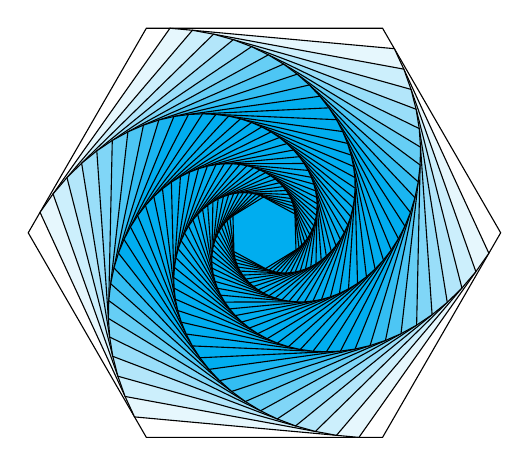
\begin{tikzpicture}
		\def\couleur{cyan}
		\path[coordinate] (0,0)  coordinate(A)
		++( 120:3cm) coordinate(B)
		++(60:3cm) coordinate(C)
		++(0:3cm) coordinate(D)
		++(-60:3cm) coordinate(E)
		++(240:3cm) coordinate(F)
		;
		\draw[fill=\couleur!\thedensity] (A) -- (B) -- (C) --(D) -- (E) -- (F)-- cycle;
		\foreach \x in {1,...,40}{%
				\pgfmathsetcounter{density}{\thedensity+10}
				\setcounter{density}{\thedensity}
				\path[coordinate] coordinate(X) at (A){};
				\path[coordinate] (A) -- (B) coordinate[pos=.10](A)
				-- (C) coordinate[pos=.10](B)
				-- (D) coordinate[pos=.10](C)
				-- (E) coordinate[pos=.10](D)
				-- (F) coordinate[pos=.10](E)
				-- (X) coordinate[pos=.10](F);
				\draw[fill=\couleur!\thedensity] (A)--(B)--(C)-- (D) --(E) -- (F) -- cycle;
			}
	\end{tikzpicture}

	\vspace{0.3cm}
	From \href{http://www.texample.net/tikz/examples/rotated-polygons/}{texample.net}.

\end{frame}


\begin{frame}[fragile]{Fig 2}

	\setcounter{density}{20}
	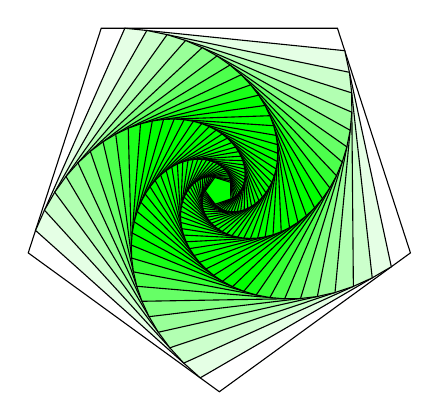
\begin{tikzpicture}
		\def\couleur{green}
		\path[coordinate] (0,0)  coordinate(A)
		++( 144:3cm) coordinate(B)
		++(72:3cm) coordinate(C)
		++(0:3cm) coordinate(D)
		++(-72:3cm) coordinate(E)
		;
		\draw[fill=\couleur!\thedensity] (A) -- (B) -- (C) --(D) -- (E) --  cycle;
		\foreach \x in {1,...,40}{%
				\pgfmathsetcounter{density}{\thedensity+10}
				\setcounter{density}{\thedensity}
				\path[coordinate] coordinate(X) at (A){};
				\path[coordinate] (A) -- (B) coordinate[pos=.10](A)
				-- (C) coordinate[pos=.10](B)
				-- (D) coordinate[pos=.10](C)
				-- (E) coordinate[pos=.10](D)
				-- (X) coordinate[pos=.10](E);
				\draw[fill=\couleur!\thedensity] (A)--(B)--(C)-- (D) --(E)  -- cycle;
			}
	\end{tikzpicture}

	\vspace{0.3cm}
	From \href{http://www.texample.net/tikz/examples/rotated-polygons/}{texample.net}.

\end{frame}